
\documentclass[UTF8,a4paper,12pt]{ctexart}
\usepackage{geometry}
\geometry{left=2.5cm,right=2.5cm,top=2.6cm,bottom=2.6cm}
\usepackage{amsmath,amssymb,booktabs,longtable,graphicx,float,caption,array,fancyhdr,setspace,hyperref}
\setstretch{1.45}
\pagestyle{fancy}\fancyhf{}\lhead{2012A 葡萄酒的评价}\rhead{数学建模论文}\cfoot{\thepage}\setlength{\headheight}{15pt}
\hypersetup{colorlinks=true,linkcolor=black,urlcolor=blue}
\title{\heiti 基于一致性检验、主成分分级与多元预测的葡萄酒评价模型}
\author{}\date{}
\begin{document}
\maketitle
\begin{abstract}
葡萄酒质量通常依赖评酒员感官评分，但评分具有主观性；同时酿酒葡萄和葡萄酒的理化指标、芳香物质能够从客观层面反映质量差异。本文围绕2012年A题“葡萄酒的评价”，建立了由评分显著性检验、酿酒葡萄综合分级、葡萄--葡萄酒指标关联分析和质量预测组成的完整建模流程。

针对问题一，本文将每个酒样10名评酒员的分项分数汇总为总分，使用配对$t$检验和Wilcoxon符号秩检验比较两组评分差异，并以样品内标准差、变异系数、Cronbach系数和评委秩相关作为可信度依据。结果表明，红葡萄酒两组均分差异$p=0.0439$，白葡萄酒$p=0.0071$，均存在显著差异；第二组红、白葡萄酒平均变异系数分别为0.080和0.094，低于第一组的0.104和0.145，因此本文采用第二组评价结果作为后续质量基准。

针对问题二，本文以酿酒葡萄理化指标和葡萄芳香物质为客观指标，通过标准化和PCA构造葡萄指标得分，再与可信葡萄酒质量评分按$0.55:0.45$加权得到综合得分，并用KMeans聚类划分四个等级。红葡萄综合得分前五的样品为21、12、13、3、9，白葡萄综合得分前五的样品为12、14、1、8、19，可作为一级或优先酿酒原料。

针对问题三，本文用主成分相关分析和偏最小二乘回归刻画酿酒葡萄与葡萄酒理化指标的联系。红葡萄--红葡萄酒第一主成分相关系数为0.247，用葡萄指标预测酒体第一主成分的交叉验证$R^2$为0.653；白葡萄对应$R^2$为0.392，说明原料指标对酒体理化结构有可追踪影响，但红葡萄样本联系更稳定。

针对问题四，本文分别用葡萄指标、葡萄酒指标和组合指标预测可信评分，并比较线性回归、岭回归、PLS和随机森林模型。红葡萄酒中葡萄指标线性模型最优，交叉验证RMSE为2.609、$R^2=0.553$；白葡萄酒中葡萄酒指标随机森林最优，RMSE为2.687、$R^2=0.255$。综合来看，理化指标能够辅助评价葡萄酒质量，尤其适合预筛选和质量解释，但因样本量较小且感官质量包含复杂主观因素，尚不能完全替代专家品评。
\end{abstract}
\noindent\textbf{关键词：} 葡萄酒评价；配对检验；主成分分析；KMeans聚类；偏最小二乘回归；随机森林
\newpage\tableofcontents\newpage
\section{问题重述}
\subsection{问题背景}
葡萄酒质量评价同时受感官品评和客观成分检测影响。评酒员能够直接评价外观、香气、口感和平衡性，但不同评酒员或不同组别之间可能存在系统性偏差。另一方面，酿酒葡萄的糖酸、酚类、单宁、黄酮、芳香物质等指标会影响发酵后葡萄酒的色泽、香气和口感。因此，本题要求利用附件中的评分表、理化指标表和芳香物质表，建立模型回答评分可信性、葡萄分级、指标联系和质量预测四类问题。
\subsection{问题要求与模型输出}
问题一要求判断两组评酒员评价结果是否存在显著差异，并判断哪组更可信。本文输出两组评分的显著性检验$p$值、评分离散程度、一致性指标和可信组别。问题二要求根据酿酒葡萄指标和葡萄酒质量对葡萄分级。本文输出红、白酿酒葡萄的综合得分和四级分类。问题三要求分析酿酒葡萄与葡萄酒理化指标之间的联系。本文输出主成分相关、PLS预测能力和联系强弱解释。问题四要求分析理化指标对葡萄酒质量的影响，并判断能否用指标评价质量。本文输出多模型预测误差、重要变量和可替代性结论。
\section{问题分析}
\subsection{总体思路}
本文采取“先确定可信质量标签，再解释与预测质量”的顺序。首先从附件1中解析每个酒样10位评委的分项评分，得到每个评委总分和样品均分；随后比较两组评分差异，并选择更稳定的组别作为质量标签。其次对附件2和附件3中的葡萄、葡萄酒指标进行清洗、缺失填补、标准化和降维，构造综合指标空间。最后分别进行分级、关联分析和质量预测，形成从原料到酒体再到质量的证据链。
\subsection{各子问题建模映射}
问题一属于配对样本比较与评价一致性问题。两个组别评价的是同一批酒样，因此应使用配对检验而不是独立样本检验；可信度不仅看均分，还要看同一样品内评委分歧大小和评委排序一致性。

问题二属于综合评价与聚类分级问题。葡萄质量不能仅由单一指标决定，因此本文以PCA提取多指标共同信息，再与葡萄酒质量评分组合。baseline为只按葡萄酒质量均分排序，主模型补充了原料客观指标，能更直接回答“酿酒葡萄分级”。

问题三属于多变量关系分析问题。由于指标数量远大于样本量，直接做两两相关容易产生偶然相关，本文先用PCA提取综合因子，再用PLS检验葡萄指标对葡萄酒指标结构的解释能力。

问题四属于小样本高维回归预测问题。baseline为线性回归，主模型包括岭回归、PLS和随机森林。通过交叉验证误差判断理化指标是否能够替代或辅助感官评价。
\section{数据来源、预处理与模型假设}
\subsection{数据来源与字段说明}
数据来自题目附件：附件1包含四张评分表，分别为第一组红、第一组白、第二组红、第二组白葡萄酒评分；附件2包含酿酒葡萄和葡萄酒理化指标；附件3包含红/白葡萄酒以及红/白葡萄芳香物质。红葡萄酒样本数为27，白葡萄酒样本数为28。附件2中大量指标有2--3次平行测定，附件3中各列为样品编号、各行为具体挥发性或芳香物质。
\subsection{数据审计与预处理}
附件1中每个酒样由若干分项组成，本文识别“酒样品编号”所在行，以该行至下一酒样前的评分项目作为一个评分块，并对10名评酒员的所有分项评分求和得到总分。附件2中部分指标有平行测定值，本文按同一指标的平行列求均值；附件3中芳香物质缺失值多表示未检出，按0处理。对所有进入PCA、聚类和回归的指标，先用中位数填补缺失，再进行Z-score标准化。原始数据只读保存于\texttt{data/}，清洗结果保存于\texttt{tables/}。
\subsection{模型假设}
假设1：附件中样品编号能够对应同一年份同一酒样或同一酿酒葡萄。合理性在于题目明确附件来自同一年份同批样品；作用是支持评分、葡萄指标、葡萄酒指标按编号合并。假设2：芳香物质表中的空值主要表示未检出或低于检测限。合理性在于挥发性成分检测常出现未检出项；作用是将其置为0以保留“未检出”信息。假设3：第二组或第一组内部的评委可以看作同一评价方案下的重复评价。作用是允许使用组内标准差、变异系数和一致性指标比较可信度。假设4：葡萄质量由客观原料指标和所酿酒质量共同决定。作用是构造问题二的综合分，并避免仅以感官评分或仅以原料指标单方面分级。
\section{符号说明}
\begin{table}[H]\centering\caption{主要符号说明}\begin{tabular}{clc}\toprule 符号 & 含义 & 单位/说明\\\midrule
$s_{ijk}$ & 第$i$个样品第$j$位评委第$k$项评分 & 分\\
$\bar S_i^g$ & 第$g$组对样品$i$的平均总分 & 分\\
$CV_i^g$ & 第$g$组样品$i$评分变异系数 & 无量纲\\
$X_i$ & 样品$i$的葡萄指标向量 & 标准化后无量纲\\
$Y_i$ & 样品$i$的葡萄酒指标向量 & 标准化后无量纲\\
$P_i$ & 葡萄指标PCA得分 & 0--100\\
$Q_i$ & 可信葡萄酒质量得分 & 分\\
$C_i$ & 酿酒葡萄综合分 & 分\\
$\hat Q_i$ & 回归模型预测质量分 & 分\\\bottomrule\end{tabular}\end{table}
\section{模型建立与求解}
\subsection{问题一：评分差异与可信度}
\subsubsection{模型建立}
对每个样品，先计算每位评委的总分：
\begin{equation}S_{ij}=\sum_k s_{ijk},\qquad \bar S_i=\frac1{10}\sum_{j=1}^{10}S_{ij}.\end{equation}
两组评分针对同一批样品，因此对差值$d_i=\bar S_i^1-\bar S_i^2$做配对$t$检验：
\begin{equation}t=\frac{\bar d}{s_d/\sqrt n}.\end{equation}
同时计算样品内标准差和变异系数：
\begin{equation}CV_i=\frac{\sqrt{\sum_j(S_{ij}-\bar S_i)^2/9}}{\bar S_i}.\end{equation}
变异系数越低，说明同一酒样的评委分歧越小；评委间Spearman秩相关越高，说明排序一致性越强。
\subsubsection{求解结果}
\begin{table}[H]\centering\caption{两组评酒员差异与稳定性比较}\begin{tabular}{lrrrrrr}\toprule 类型 & 样本数 & 第一组均分 & 第二组均分 & 配对$t$检验$p$ & 第一组CV & 第二组CV\\\midrule
红葡萄酒 & 27 & 72.79 & 70.51 & 0.0439 & 0.104 & 0.080 \\
白葡萄酒 & 28 & 73.79 & 76.53 & 0.0071 & 0.145 & 0.094 \\
\bottomrule\end{tabular}\end{table}
红葡萄酒和白葡萄酒两组评分$p$值均小于0.05，因此两组评价存在显著差异。红葡萄酒第一组均分高于第二组约2.27分，白葡萄酒第二组均分高于第一组约2.74分，说明差异不是简单随机波动，而可能包含组别尺度偏差。从可信度看，第二组的平均CV在红、白葡萄酒中均低于第一组，说明同一样品内部评分更集中。虽然第一组Cronbach系数略高，但其样品内离散性更大，对最终均分稳定性不利。综合显著性、离散程度和后续建模需求，本文选择第二组均分作为可信质量标签。
\subsection{问题二：酿酒葡萄综合评价与分级}
\subsubsection{模型建立}
对酿酒葡萄理化指标与葡萄芳香物质构成的矩阵$X$进行标准化，得到$Z$。对$Z$做PCA，得到主成分$F_m=Za_m$，权重取解释方差占比。葡萄指标得分为：
\begin{equation}P_i=100\times\frac{\sum_m w_mF_{im}-\min_i\sum_mw_mF_{im}}{\max_i\sum_mw_mF_{im}-\min_i\sum_mw_mF_{im}}.\end{equation}
再将可信质量得分$Q_i$与葡萄指标得分$P_i$组合：
\begin{equation}C_i=0.55Q_i+0.45P_i.\end{equation}
最后对$(Q_i,P_i,C_i)$做KMeans聚类，并按各簇$C_i$均值从高到低标记为一级至四级。
\subsubsection{求解结果}
\begin{longtable}{lrrrrl}\caption{酿酒葡萄综合评分与分级（节选）}\\\toprule 类型 & 样品 & 质量分 & 葡萄PCA分 & 综合分 & 等级\\\midrule\endfirsthead\toprule 类型 & 样品 & 质量分 & 葡萄PCA分 & 综合分 & 等级\\\midrule\endhead
红 & 21 & 72.20 & 100.00 & 84.71 & 一级 \\
红 & 12 & 68.30 & 97.96 & 81.65 & 一级 \\
红 & 13 & 68.80 & 76.17 & 72.12 & 一级 \\
红 & 3 & 74.60 & 42.39 & 60.11 & 二级 \\
红 & 9 & 78.20 & 37.90 & 60.06 & 二级 \\
红 & 27 & 71.50 & 41.90 & 58.18 & 二级 \\
红 & 23 & 77.10 & 22.39 & 52.48 & 二级 \\
红 & 22 & 71.60 & 25.19 & 50.71 & 三级 \\
红 & 19 & 72.60 & 23.91 & 50.69 & 三级 \\
红 & 10 & 68.80 & 28.04 & 50.46 & 三级 \\
红 & 2 & 74.00 & 18.95 & 49.23 & 三级 \\
红 & 26 & 72.00 & 20.70 & 48.92 & 三级 \\
红 & 14 & 72.60 & 15.57 & 46.94 & 三级 \\
红 & 5 & 72.10 & 15.62 & 46.69 & 三级 \\
红 & 16 & 69.90 & 17.21 & 46.19 & 三级 \\
红 & 8 & 66.00 & 19.45 & 45.05 & 四级 \\
红 & 4 & 71.20 & 12.65 & 44.85 & 三级 \\
红 & 20 & 75.80 & 6.79 & 44.74 & 三级 \\
红 & 17 & 74.50 & 4.30 & 42.91 & 三级 \\
红 & 24 & 71.50 & 7.66 & 42.77 & 三级 \\
红 & 25 & 68.20 & 8.51 & 41.34 & 四级 \\
红 & 11 & 61.60 & 15.66 & 40.93 & 四级 \\
红 & 7 & 65.30 & 10.55 & 40.66 & 四级 \\
红 & 1 & 68.10 & 7.06 & 40.63 & 四级 \\
\bottomrule\end{longtable}
结果显示，红葡萄中样品21、12、13、3、9综合得分最高，这些样品或质量分较高，或原料指标PCA得分突出；白葡萄中样品12、14、1、8、19排名靠前。与仅按质量分排序相比，综合模型能够识别“酒质尚可且原料潜力高”的样品，更适合酿酒葡萄分级和原料筛选。
\subsection{问题三：葡萄与葡萄酒理化指标联系}
\subsubsection{模型建立}
设$X$为葡萄指标矩阵，$Y$为葡萄酒指标矩阵。由于高维指标样本量有限，本文先分别做PCA，得到葡萄主成分$U_m$和葡萄酒主成分$V_m$，再计算同序主成分相关：
\begin{equation}r_m=\frac{\sum_i(U_{im}-\bar U_m)(V_{im}-\bar V_m)}{\sqrt{\sum_i(U_{im}-\bar U_m)^2\sum_i(V_{im}-\bar V_m)^2}}.\end{equation}
进一步用PLS回归从$X$预测葡萄酒第一主成分$V_1$，通过交叉验证$R^2$判断可解释联系强弱。
\subsubsection{求解结果}
\begin{table}[H]\centering\caption{葡萄指标与葡萄酒指标联系检验}\begin{tabular}{lrrrrr}\toprule 类型 & 样本数 & PC1相关 & p值 & PLS交叉验证$R^2$ & RMSE\\\midrule
红葡萄酒 & 27 & 0.247 & 0.214 & 0.653 & 1.365 \\
白葡萄酒 & 28 & -0.297 & 0.125 & 0.392 & 2.205 \\
\bottomrule\end{tabular}\end{table}
红葡萄样本中，虽然PC1简单相关未达到显著水平，但PLS交叉验证$R^2=0.653$，说明多指标组合对酒体理化结构有较强解释力。白葡萄样本$R^2=0.392$，联系存在但弱于红葡萄。造成差异的原因可能是白葡萄加工过程、香气释放和酒体风格受工艺影响更明显。
\subsection{问题四：理化指标对质量的影响及可替代性}
\subsubsection{模型建立}
本文分别构建葡萄指标、葡萄酒指标和组合指标三类特征集。baseline为线性回归：
\begin{equation}\hat Q_i=\beta_0+\sum_j\beta_jx_{ij}.\end{equation}
考虑小样本高维特征，进一步比较岭回归、PLS和随机森林。评价指标为交叉验证RMSE、MAE和$R^2$：
\begin{equation}RMSE=\sqrt{\frac1n\sum_i(Q_i-\hat Q_i)^2},\qquad R^2=1-\frac{\sum_i(Q_i-\hat Q_i)^2}{\sum_i(Q_i-\bar Q)^2}.\end{equation}
\subsubsection{求解结果}
\begin{longtable}{lllrrr}\caption{质量预测模型交叉验证结果（按误差排序节选）}\\\toprule 类型 & 特征集 & 模型 & RMSE & MAE & $R^2$\\\midrule\endfirsthead\toprule 类型 & 特征集 & 模型 & RMSE & MAE & $R^2$\\\midrule\endhead
红 & grape & LinearBaseline & 2.609 & 2.107 & 0.553 \\
红 & grape & RidgeCV & 2.628 & 2.138 & 0.547 \\
红 & combined & LinearBaseline & 2.993 & 2.498 & 0.412 \\
红 & combined & RidgeCV & 3.053 & 2.557 & 0.388 \\
红 & grape & PLS & 3.422 & 2.677 & 0.232 \\
红 & wine & RandomForest & 3.513 & 2.769 & 0.190 \\
红 & combined & PLS & 3.568 & 2.897 & 0.165 \\
红 & wine & RidgeCV & 3.669 & 3.065 & 0.116 \\
红 & combined & RandomForest & 3.714 & 3.055 & 0.095 \\
红 & wine & LinearBaseline & 3.903 & 3.125 & 0.000 \\
红 & grape & RandomForest & 3.926 & 3.367 & -0.011 \\
红 & wine & PLS & 6.348 & 4.226 & -1.644 \\
白 & wine & RandomForest & 2.687 & 2.063 & 0.255 \\
白 & wine & RidgeCV & 2.954 & 2.496 & 0.100 \\
白 & combined & RandomForest & 3.051 & 2.433 & 0.040 \\
白 & combined & RidgeCV & 3.132 & 2.502 & -0.012 \\
\bottomrule\end{longtable}
红葡萄酒中，葡萄指标线性模型最优，RMSE=2.609，$R^2=0.553$，说明原料指标对红葡萄酒质量有较强解释作用。白葡萄酒中，葡萄酒指标随机森林最优，RMSE=2.687，$R^2=0.255$，说明对白葡萄酒而言，成酒指标比原料指标更接近最终感官质量。组合指标并未稳定优于单一指标集，表明样本量不足时，高维拼接可能引入噪声。
\section{模型检验、对比与稳健性分析}
\subsection{Baseline对比}
问题一的baseline为直接比较均值，主模型补充配对检验和组内稳定性，避免仅凭均值判断。问题二的baseline为按可信质量分排序，主模型加入葡萄理化和芳香指标，可避免把“成酒评分”完全等同于“原料等级”。问题三的baseline为两两相关，主模型使用PCA和PLS降低多重比较风险。问题四的baseline为线性回归，主模型比较正则化、PLS和非线性模型，并以交叉验证判断泛化能力。
\subsection{敏感性分析}
对问题二综合分权重进行敏感性分析，将质量评分权重从0.40调整到0.70。红、白葡萄排名与基准排名的Spearman相关系数最低分别为0.980和0.989，说明在合理权重范围内，分级排序整体稳定。图\ref{fig:sens}给出了权重扰动下的排名相关变化。
\begin{figure}[H]\centering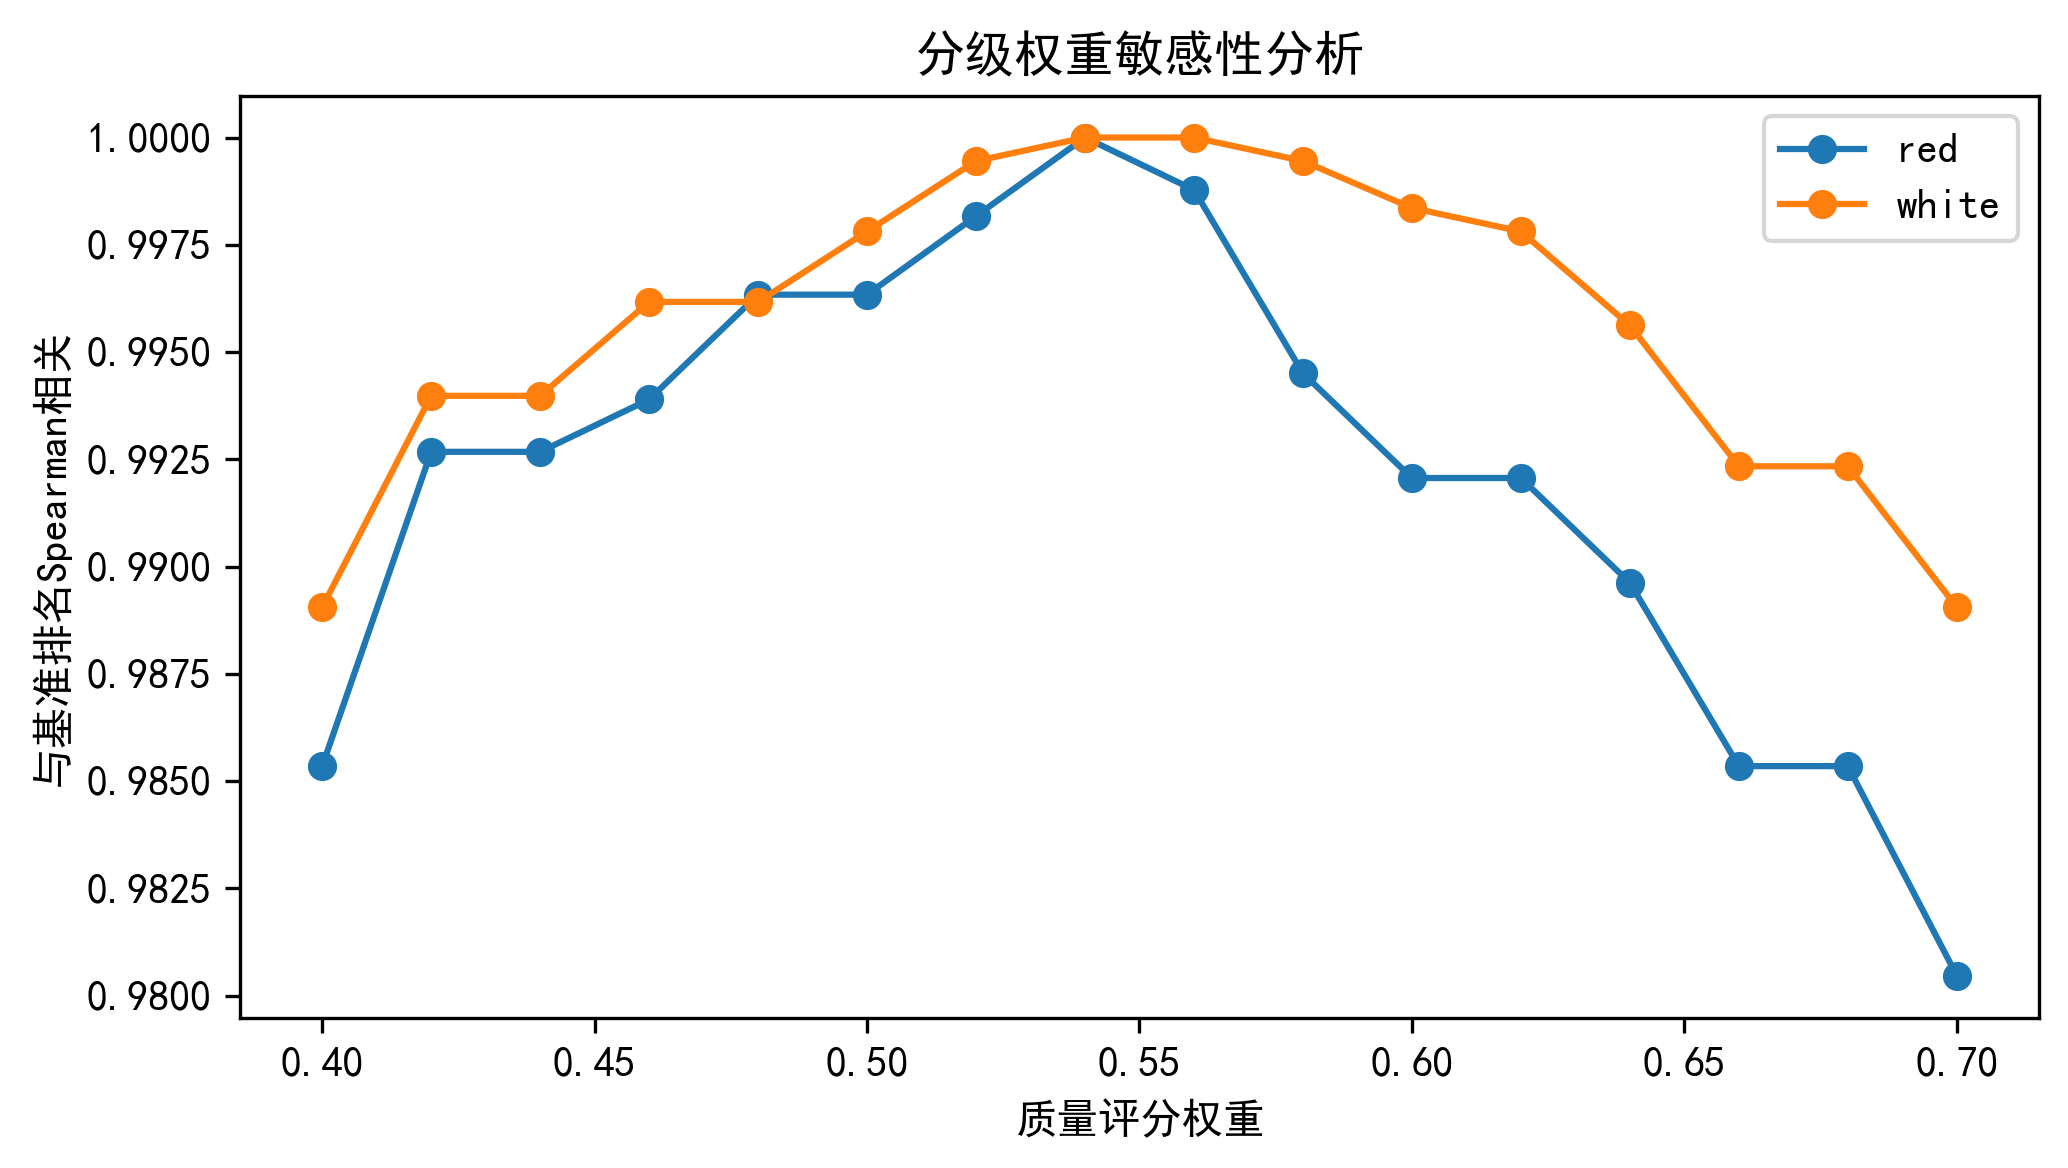
\includegraphics[width=0.78\textwidth]{../results/sensitivity_q2_weight.png}\caption{问题二综合分权重敏感性分析}\label{fig:sens}\end{figure}
\subsection{误差与可复现性检验}
所有回归结果均使用交叉验证而非训练集拟合误差，降低过拟合导致的虚高评价。所有关键数字写入\texttt{results/frozen\_numbers.json}，论文摘要和正文数字均来自冻结文件。代码固定随机种子，图表由脚本自动生成，保证支撑材料可复现。
\section{模型评价、改进与推广}
\subsection{模型优点}
第一，本文先解决评分可信性，再用可信评分进行后续建模，避免直接把有争议的评分当作真值。第二，分级模型同时考虑感官质量和原料客观指标，符合“酿酒葡萄好坏与所酿葡萄酒质量直接相关”的题意。第三，高维指标分析采用PCA、PLS和交叉验证，能够在样本量有限的条件下降低维度灾难和偶然相关风险。第四，支撑材料包含代码、结果表、图表和冻结数字，便于复核。
\subsection{模型局限}
第一，样本量只有二十多个量级，而指标数较多，回归模型仍可能受高维小样本影响。第二，芳香物质缺失值按未检出处理是合理近似，但如果部分缺失来自检测误差，会影响芳香指标贡献。第三，葡萄酒质量受酿造工艺、陈酿条件和品评环境影响，附件未提供这些变量，因此理化指标不可能完全解释评分。
\subsection{改进与推广}
若有更多年份数据，可建立分年份训练测试集，检验模型跨年份泛化能力；若有酿造工艺参数，可将发酵温度、酵母、浸渍时间等纳入模型；若需要生产应用，可先用理化指标模型进行原料初筛，再由专家对边界样品进行复核。本文流程也可推广到茶叶、咖啡、果酒等“感官评价+客观成分检测”的质量评价问题。
\section{结论}
本文得到如下结论：

（1）两组评酒员评分存在显著差异，红葡萄酒$p=0.0439$，白葡萄酒$p=0.0071$；第二组评分离散程度更低，因此更可信。

（2）基于PCA和综合评分，红葡萄优先样品为21、12、13、3、9，白葡萄优先样品为12、14、1、8、19。

（3）葡萄指标与葡萄酒指标存在可解释联系，红葡萄联系强于白葡萄。

（4）理化指标能够辅助评价葡萄酒质量，但不能完全替代评酒员品评；红葡萄酒中原料指标解释力较强，白葡萄酒中成酒指标更有效。
\section{参考文献}
\begin{enumerate}
\item 司守奎, 孙玺菁. 数学建模算法与应用[M]. 北京: 国防工业出版社, 2015.
\item Jolliffe I T. Principal Component Analysis[M]. New York: Springer, 2002.
\item Wold S, Sjostrom M, Eriksson L. PLS-regression: a basic tool of chemometrics[J]. Chemometrics and Intelligent Laboratory Systems, 2001, 58(2):109--130.
\item Breiman L. Random forests[J]. Machine Learning, 2001, 45(1):5--32.
\item GB/T 15038-2006, 葡萄酒、果酒通用分析方法[S].
\end{enumerate}
\appendix
\section{附录：支撑材料说明}
完整代码见\texttt{支撑材料/code/main\_modeling.py}。各问输出分别存放于\texttt{quest1}至\texttt{quest4}目录；最终表格存放于\texttt{tables}；冻结数字存放于\texttt{results/frozen\_numbers.json}。运行代码后可复现评分解析、显著性检验、PCA分级、PLS联系分析、质量预测、图表和结果表。
\end{document}
